\label{fs}
%%%%%%%%%%%%%%%%%%%%%%%%%%%%%%%%%%%%%%%%%%%%%%%%%%%%%%%%%%%%%%%%%%
%%%%%%%%%%%%%%%%%%%%%%%%%%%%%%%%%%%%%%%%%%%%%%%%%%%%%%%%%%%%%%%%%%

\subsection{Introduction}
Dans le chapitre \ref{peripherals} qui traite le sujet des périphériques, nous
avons vu très brièvement qu'un processeur \acrshort{IA-32} peut avoir un controlleur
de disque dur. Actuellement, tout le \textit{kernel} et ses dépendances sont
stockés dans la \acrshort{ram}. Si on veut plus tard exécuter des programmes utilisateur
ou lire et écrire des fichiers texte, il est nécessaire d'avoir un disque dur.
Un disque dur permet de stocker des fichiers qui pourront être lus par l'\acrshort{os}
si besoin. Pour rendre possible la gestion de plusieurs fichiers dans un disque
dur, ce dernier doit contenir un système de fichiers. Un système de fichiers va
organiser les fichiers ajoutés au disque dur d'une manière bien précise afin
de les retrouver rapidement. Pour rappel, notre machine est émulée par QEMU.
Comme pour tous les autres périphériques gérés par notre \acrshort{os}, QEMU
émule aussi un disque dur. Ce disque dur est vierge, il faut donc lui mettre
un système de fichiers. Une option de QEMU permet de mettre un système de fichiers
dans le disque dur émulé à partir d'un fichier image. Ci-dessous la modification
apportée à l'exécution du \textit{kernel}.

\begin{minted}[fontsize=\footnotesize,tabsize=4]{text}
$ qemu-system-i386 -cdrom kernel.iso -hda fs.img
\end{minted}

L'option  \mintinline{text}{-cdrom} spécifie l'image \acrshort{iso} contenant
le \textit{kernel} (voir partie \ref{iso}) et l'option \mintinline{text}{-hda} indique
que le fichier image contenant le système de fichiers sera chargé dans le premier
disque dur. La gestion d'un système de fichiers par le \textit{kernel} s'est donc
déroulé en deux étapes. Il a d'abord fallut créer un système de fichiers simple
puis implémenter les \textit{drivers} au niveau du \textit{kernel} pour le lire.
Le système de fichiers utilisé par notre \textit{kernel} est inspiré de \acrshort{fat}. \\

Un système de fichiers \acrshort{fat} est divisé en blocs de même taille. Ces blocs,
aussi appelés \textit{clusters} sont eux-mêmes divisés en secteurs dont la taille
est fixe (512 octets). A noter qu'un \textit{cluster} peut avoir la même taille
en octets qu'un secteur. Le système de fichiers gère une table indiquant si un
\textit{cluster} est alloué. Cette table, appelée table d'allocation de fichiers
(ou \textit{file allocation table} en anglais) est une carte où chaque entrée
représente un \textit{cluster}. Une entrée dans la table d'allocations a une taille
différente en fonction du type de \acrshort{fat}. La taille maximale du système
de fichiers en nombre de \textit{clusters} dépend de la taille de cette entrée en
bits. Si par exemple une entrée dans la table d'allocation fait 12 bits, le système
de fichiers pourra allouer un maximum de 4096 \textit{clusters} ($2^{12} = 4096$).
Il existe plusieurs versions du système de fichiers \acrshort{fat} qui se
différencient par la taille de leurs entrées dans la table d'allocation.
\acrshort{fat}12 a des entrées de 12 bits, \acrshort{fat}16 des entrées de 16 bits
et \acrshort{fat}32 des entrées de 32 bits. La \acrshort{fat} utilisée par notre
\textit{kernel} a des entrées de huit bits, elle serait donc une \acrshort{fat}8.

\begin{figure}[!h]
  \centering
  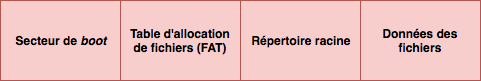
\includegraphics[scale=0.65]{images/fat.png}
  \caption{Structure d'un système de fichiers de type \acrshort{fat}}
  \label{fat}
\end{figure}

La figure \ref{fat} montre de manière simplifiée la structure d'un système de fichiers
\acrshort{fat}. Le système de fichiers réalisé s'inspire beaucoup de cette structure.

%%%%%%%%%%%%%%%%%%%%%%%%%%%%%%%%%%%%%%%%%%%%%%%%%%%%%%%%%%%%%%%%%%
%%%%%%%%%%%%%%%%%%%%%%%%%%%%%%%%%%%%%%%%%%%%%%%%%%%%%%%%%%%%%%%%%%

\subsection{Structure}
Notre système de fichiers a une structure similaire à \acrshort{fat} mais en plus
simplifiée. Dans \acrshort{fat}, les 512 premiers octets sont reservés au secteur
de \textit{boot}. Ce secteur contient toutes les informations sur le système de
fichiers comme la taille d'un secteur, la taille d'un \textit{cluster}, le type
de \acrshort{fat} (\acrshort{fat}12/16/32), etc. Dans notre système de fichiers,
l'équivalent est le \textit{superblock}. Sa taille est aussi de 512 octets mais
actuellement seulement 23 octets sont utilisés. Ci-dessous, les détails sur le
\textit{superblock}.

\begin{center}
	\scalebox{1}{
		\begin{tabular}{| c | c | c | C{5cm} |}
			\hline
			Position (octets) & Taille (octets) & Nom & Description \\ \hline
			11 & 2 & \mintinline{rust}{sector_size} & Taille d'un secteur en octets \\ \hline
			13 & 1 & \mintinline{rust}{block_size} & Taille d'un bloc en secteurs \\ \hline
			36 & 4 & \mintinline{rust}{fat_size} & Taille de la table d'allocation en blocs \\ \hline
			42 & 2 & \mintinline{rust}{version} & Version du système \\ \hline
			44 & 4 & \mintinline{rust}{root_entry} & Indice du bloc contenant les métadonnées \\ \hline
            82 & 8 & \mintinline{rust}{label} & Nom du système de fichiers \\ \hline
            510 & 2 & \mintinline{rust}{signature} & Signature (0x55aa) \\ \hline
		\end{tabular}
	}
    \captionof{table}{Structure du \textit{superblock}}
    \label{tab:fs:struct:superblock}
\end{center}

La table d'allocation de fichiers vient directement après le \textit{superblock}.
Comme expliqué dans la partie précédente, son fonctionnement est similaire en tout
point à celui de \acrshort{fat} à la différence que les entrées ont une taille fixe
de huit bits. De plus, dans un système de fichiers \acrshort{fat}, il peut y avoir
plusieurs tables d'allocation contrairement à notre système qui en aura toujours
une seule. Vient ensuite une zone alignée sur la taille d'un bloc (ou \textit{cluster})
contenant toutes les métadonnées des fichiers. Cet espace est aligné car il faut
qu'il commence au début d'un bloc afin de le retrouver à partir du \textit{superblock}.
La taille de cet espace est d'un bloc et ne peut pour le moment pas être agrandi
(contrairement à \acrshort{fat} où un nouveau \textit{cluster} est alloué au besoin).
Chaque entrée dans cet espace est une structure de 32 octets contenant notamment
l'indice du premier bloc de données du fichier (voir le tableau ci-dessous pour
plus de détails sur la structure d'une entrée).

\begin{center}
	\scalebox{1}{
		\begin{tabular}{| c | c | c |}
			\hline
			Taille (octets) & Nom & Description \\ \hline
			26 & \mintinline{rust}{name} & Nom du fichier \\ \hline
			2 & \mintinline{rust}{start} & Indice du premier bloc de données \\ \hline
			4 & \mintinline{rust}{size} & Taille du fichier \\ \hline
		\end{tabular}
	}
    \captionof{table}{Structure d'une entrée dans l'espace de métadonnées}
    \label{tab:fs:struct:entry}
\end{center}

Les blocs de données sont situés juste après le bloc de métadonnées. A noter de
plus que notre système de fichiers n'est pas hiérarchique. Tous les fichiers sont
ajoutés à la racine du système (pas de répertoires). A partir de ces structures,
ont peut facilement accéder à un fichier dans le disque. Les informations contenus
dans le \textit{superblock} permettent de localiser le bloc de métadonnées. Le
fichier demandé est trouvé en parcourant ce bloc et son premier bloc de données
peut ainsi être lu. Il reste toujours un problème si le fichier a une taille supérieure
à la taille d'un bloc. C'est là que la table d'allocation peut être
utilisée. En effet, l'entrée de la table d'allocation correspondant au bloc
de données peut soit pointer sur le bloc suivant, soit indiquer que ce bloc est
le dernier de la chaîne. \newpage

\begin{figure}[!h]
  \centering
  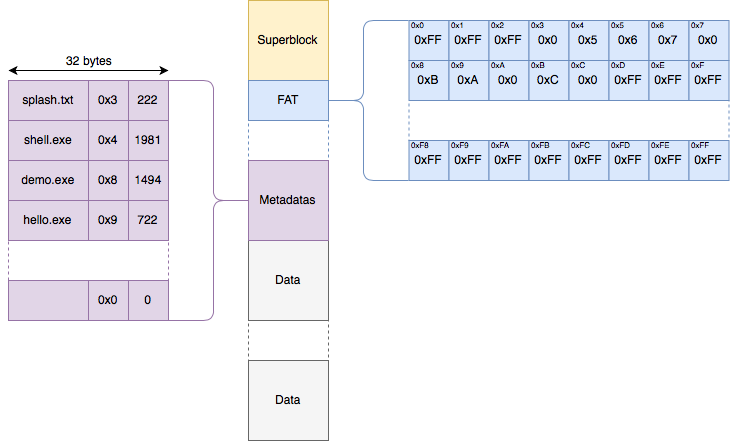
\includegraphics[scale=0.6]{images/microfs.png}
  \caption{Système de fichiers de l'\acrshort{os}}
  \label{microfs}
\end{figure}

La figure \ref{microfs} donne un exemple de contenu du système
de fichiers développé. Dans cet exemple, la taille d'un bloc est la même que la
taille d'un secteur. Le système de fichiers contient quatre fichiers. Le premier,
\mintinline{text}{splash.txt}, rentre dans un seul bloc. La chaîne d'allocation
s'arrête dès la première entrée avec un 0x0 écrit dans l'entrée 0x3 de la table
d'allocation. Prenons maintenant le deuxième fichier, \mintinline{text}{shell.exe}.
Ce fichier a besoin de quatre blocs pour être stocké. Dans la table d'allocation,
on voit que le premier bloc de ce fichier (d'indice 0x4) pointe sur le bloc
d'indice 0x5. En suivant ainsi la chaîne d'allocation, on peut retrouver l'intégralité
des blocs de données à partir de leurs indices. Cet exemple montre aussi que la
\acrshort{fat} permet de stocker les fichiers de manière discontinue. Le fichier
\mintinline{text}{demo.exe} commence au bloc d'indice 0x8 mais son deuxième bloc
n'est pas à l'indice 0x9 mais à l'indice 0xB.

%%%%%%%%%%%%%%%%%%%%%%%%%%%%%%%%%%%%%%%%%%%%%%%%%%%%%%%%%%%%%%%%%%
%%%%%%%%%%%%%%%%%%%%%%%%%%%%%%%%%%%%%%%%%%%%%%%%%%%%%%%%%%%%%%%%%%

\subsection{Implémentation}
La construction du système de fichiers se fait à l'aide d'un outil externe. Cet
outil a été développé en utilisant la version standard de rust. Il s'exécute
par conséquent depuis la machine hôte et le gestionnaire de paquet de rust, cargo,
peut être utilisé normalement. L'outil développé possède deux
modes de fonctionnement. Soit à l'aide d'un menu soit directement en ligne de
commande en spécifiant certaines options. Les deux modes de fonctionnement
font exactement la même chose. Ils manipulent un fichier image donné.
Cet outil permet de créer un système de fichiers vide, d'ajouter et de supprimer
un fichier, de lister l'intégralité des fichiers contenus dans le système de fichiers et enfin
d'afficher les informations du \textit{superblock}. La gestion des arguments en
ligne de commande se fait à l'aide du paquet \mintinline{text}{clap} installé avec
cargo. Le menu avec les différentes options décrites se présente comme sur la figure
\ref{microfs_menu}. Toutes les options de ce menu peuvent aussi être appelées
directement en ligne de commande (sauf l'option \textit{save} qui sauvegarde les
modifications apportées au système de fichiers). \\ 

\begin{figure}[!h]
  \centering
  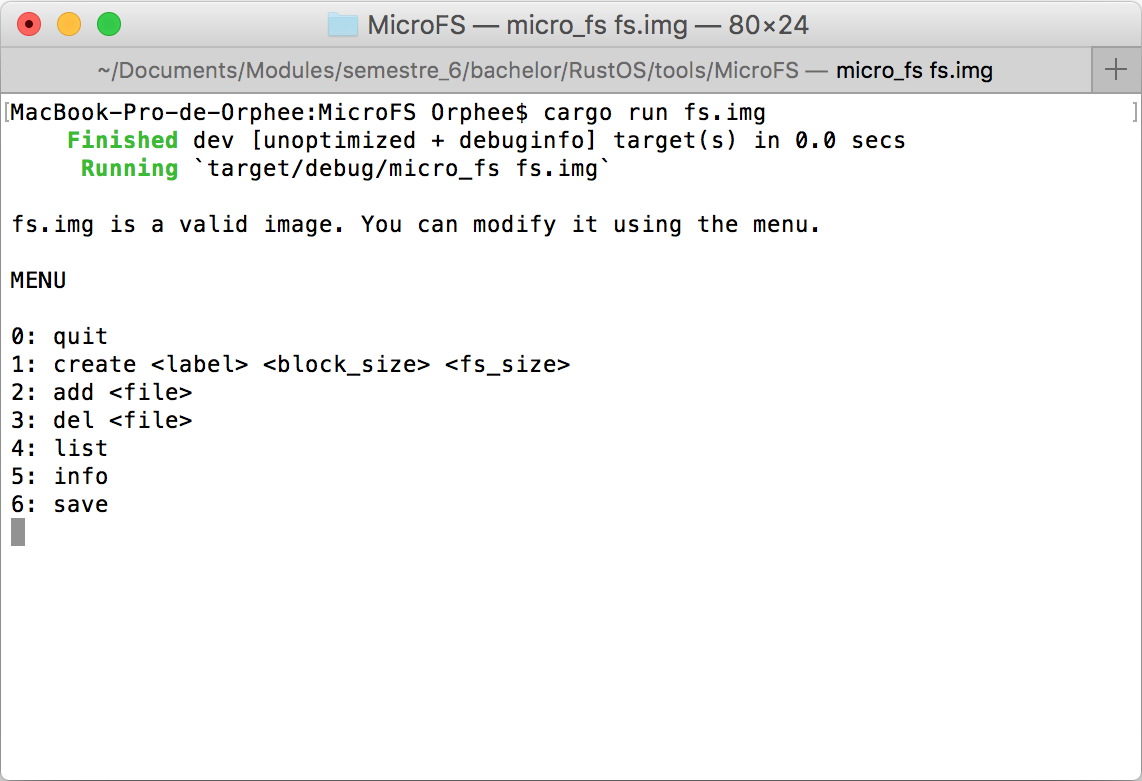
\includegraphics[scale=0.6]{images/microfs_menu.png}
  \caption{Menu du gestionnaire du système de fichiers}
  \label{microfs_menu}
\end{figure}

Ce menu est finalement très peu utilisé car nous avons besoin de créer le système
de fichiers en ligne de commande, avec le même \mintinline{text}{makefile} utilisé
pour la compilation du \textit{kernel}. Il peut quand même être pratique pour faire
des tests rapides ou avoir un retour plus visuel de la modification
du système de fichiers. Nous avons vu comment le système de fichiers était construit
dans un fichier image et aussi que ce fichier image pouvait être donné à QEMU afin
d'être chargé dans le disque dur virtuel. Il reste encore à lire dans le système
de fichiers depuis le \textit{kernel}. Pour lire dans le système de fichiers, il
faut utiliser les ports du controlleur de disque dur. QEMU peut émuler plusieurs
disques. Nous utilisons le premier dont les registres de contrôle sont aux ports
0x1f0 à 0x1f7. La lecture et l'écriture de secteurs (512 octets) du disque dur
sont fait par l'intermédiaire de ces registres. Un code d'exemple peut être trouvé
sur le site OSDev \cite{ref24}. Deux fonctions ont été implémentées pour communiquer
avec le controlleur de disque dont les prototypes sont ci-dessous.

\begin{code}
\begin{minted}[fontsize=\footnotesize,tabsize=4,frame=single,linenos]{rust}
pub fn read_sector(sector: u32, dst: *mut u16);
pub fn write_sector(sector: u32, src: *mut u16);
\end{minted}
\caption{Prototypes des fonctions d'écriture/lecture dans le disque dur}
\label{lst:fs:impl:rw}
\end{code} \bigbreak

Le système de fichiers actuel ne permet que la lecture, pas l'écriture.
Seule la première fonction est donc utilisée par le \textit{kernel}. Ce dernier
peut maintenant lire les secteurs du système de fichiers ce qui rend possible
la réalisaton d'une \acrshort{api} de gestion des fichiers contenus dans le disque dur.
Cette \acrshort{api} s'inspire de la sémantique \acrshort{posix} pour l'accès aux
fichiers (\mintinline{text}{open}, \mintinline{text}{read}, \mintinline{text}{close},
etc). Le \textit{kernel} maintient une table de descripteurs de fichiers ouverts.
Un descripteur de fichier est composé des métadonnées du fichier (structure
\mintinline{rust}{Stat}) ainsi que la position dans le flux d'octets du fichier.
Quand un fichier est ouvert avec la fonction \mintinline{text}{file_open}, un descripteur
de fichier sur huit bits est renvoyé. Ce descripteur est en fait un indice dans
la table des descripteurs. Les fonctions \mintinline{text}{file_read},
\mintinline{text}{file_close} et \mintinline{text}{file_seek} manipulent
ce descripteur de fichier. Des fonctions et structures pour itérer les fichiers
du système de fichiers ont aussi été implémentées dans cette \acrshort{api}.